\chapter{Algorithm}\label{chap:algorithm}
The algorithm followed to fulfill the required funcionality for the project is presented in this chapter. The code for the KUKA robot is contained in \lstinline[style=matlabinline]{MiniprojectCodeKUKA.m} whereas the code for the simulation in Robot Studio can be found in \lstinline[style=matlabinline]{MiniprojectCodeRobotStudio.m}. Both of these files show the same algorithm, which can be summarized as
\begin{enumerate}
	\item Identification of the Lego bricks in order to obtain its position and orientation.
	\item Check figures required and number of bricks available and number of final locations available. 
	\item If everything is correct, pick and place the bricks in their destination with subsequent operations.
\end{enumerate}
\section{Identification of the Bricks}
The goal of the brick identification algorithm is to obtain the position and orientation of the bricks so as to generate appropiate commands for the robot.

The algorithm is illustrated with an example image taken in similar conditions as in the workstation, \autoref{fig:RealLego4}. It is based on the the information of hue, saturation and value given by the representation on the image in HSV color space.

\begin{figure}[H]
	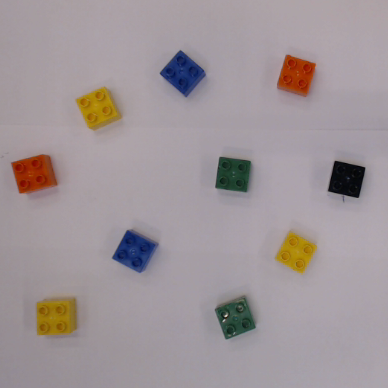
\includegraphics[width=0.25\textwidth]{figures/original.png}
	\caption{Original image that includes the color bricks to identify in random positions.}
	\label{fig:RealLego4}
\end{figure}

The first step is to convert the image to HSV color space and split into the three different channels, as seen in \autoref{list:hsv}.
%
\begin{lstlisting}[ language = Matlab,
caption  = {MATLAB code to split the image in the three HSV channels.},
label    = list:hsv ]
% Transform into HSV and separate in the different channels
hsv=rgb2hsv(original);
hue=hsv(:,:,1);
saturation=hsv(:,:,2);
value=hsv(:,:,3);
\end{lstlisting}

The common characteristic of all colored bricks is their high brightness in the saturation channel, see \autoref{fig:saturation} as they are painted with bright colors. For this reason, the saturation channel image is thresholded to find orange, yellow, green and blue bricks. The threshold applied is 0.2 in the range [0,1]. This process gives as a result the binary mask shown in \autoref{fig:colour_mask}, where the white pixel values represent the colored bricks in the original image.

\begin{figure}[H]
	\captionbox  %<--use captionbox instead if no global caption is needed
	{ 
		Saturation channel of the original image in HSV color space.              
		\label{fig:saturation}                                  
	}                                                                 
	{                                                                  
		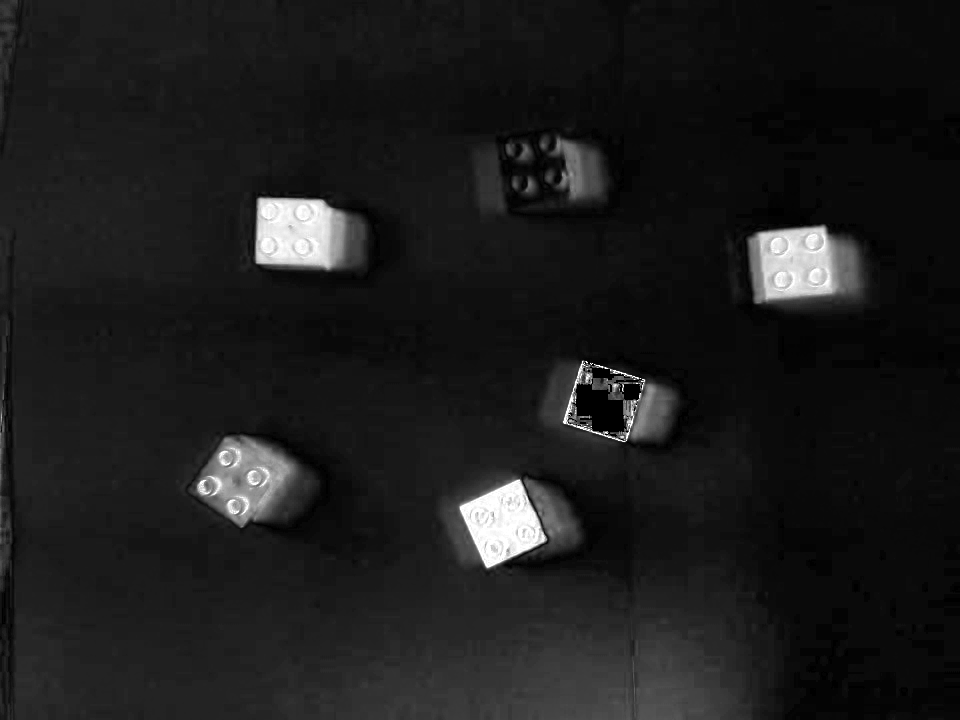
\includegraphics[width=.25\textwidth]{figures/saturation.png}         
	}                                                                    
	\hspace{5pt}                                                          
	\captionbox
	{      
		Mask for the colored bricks (orange, green, blue and yellow). 
		\label{fig:colour_mask}                                     
	}
	{
		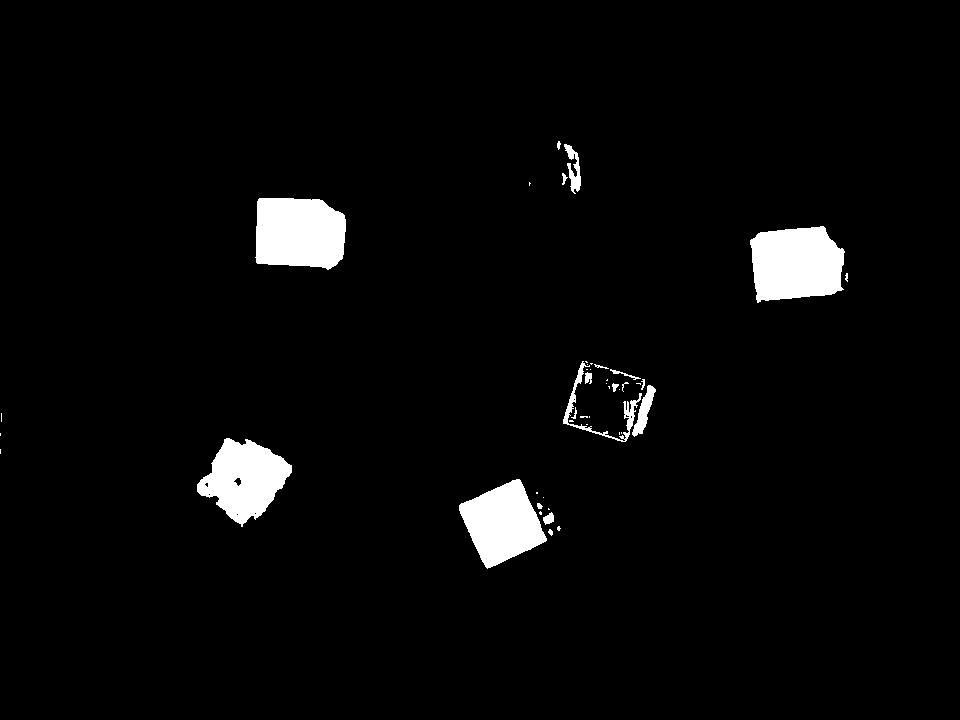
\includegraphics[width=.25\textwidth]{colour_mask.png}            
	}                                                                             
\end{figure}

The black bricks will not be detected using the saturation channel of the image. For these, the value channel is used instead. This is suitable as black has a very low brightness in this channel. This new thresholding operation takes the low value pixels and creates the mask seen in \autoref{fig:black_mask}. The threshold used is 0.2 in the range [0,1].
\begin{figure}[H]
	\captionbox  %<--use captionbox instead if no global caption is needed
	{
		Value channel of the original image in HSV color space.                
		\label{fig:value}                                  
	}                                                                 
	{       
		
		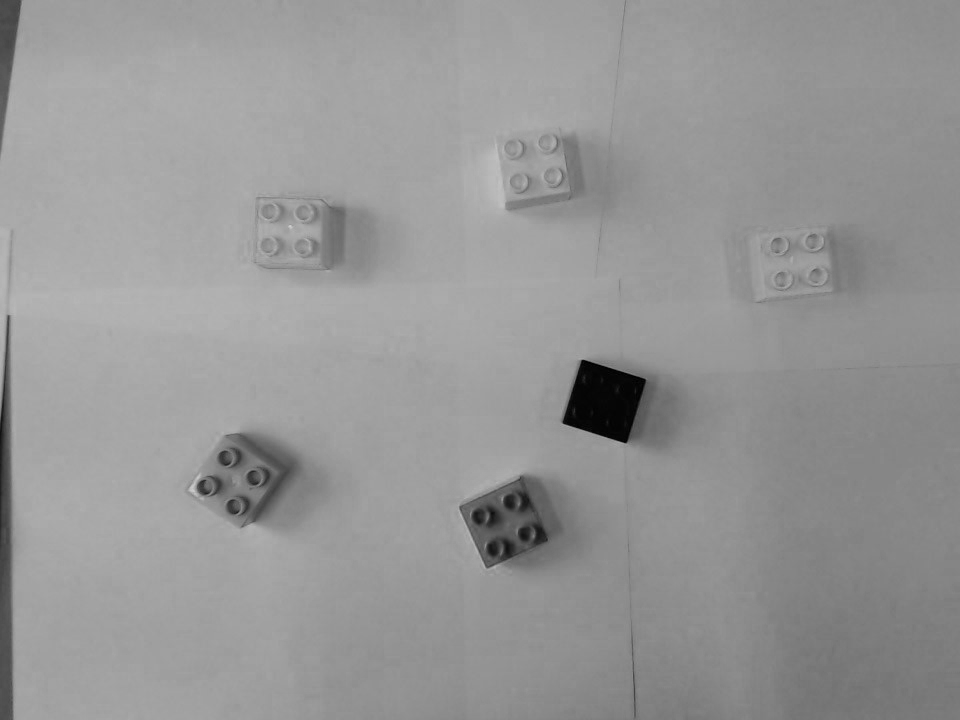
\includegraphics[width=.25\textwidth]{figures/value.png}         
	}                                                                    
	\hspace{5pt}                                                          
	\captionbox
	{  
		Mask for the black brick.
		\label{fig:black_mask}                                     
	}
	{
		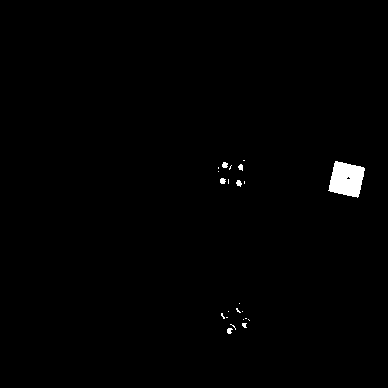
\includegraphics[width=.25\textwidth]{black_mask.png}            
	}                                                                             
\end{figure}
The masks for the colored bricks and for the black bricks are then combined resulting in \autoref{fig:final_mask}. As it is noticeable in the mask, there are holes in some of the blobs and, although noise does not appear in the image, it has a high probability of appearing in other images taken. For solving these two issues, an opening operation, followed by a closed operation removes both noise and holes, respectively. Both processes use a $5\times 5$ square kernel and the result after being applied on \autoref{fig:final_mask} can be seen in \autoref{fig:final_mask2}. 
%
\begin{figure}[H]
	\captionbox  %<--use captionbox instead if no global caption is needed
	{
		Combination of both masks before processing.             
		\label{fig:final_mask}                                  
	}                                                                 
	{                                                                  
		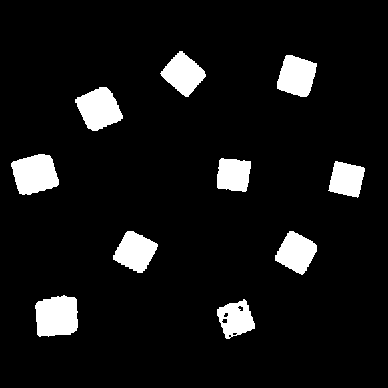
\includegraphics[width=.25\textwidth]{figures/final_mask.png}         
	}                                                                    
	\hspace{5pt}                                                          
	\captionbox
	{       
		Enhanced mask after removing noise and filling holes in the objects.
		\label{fig:final_mask2}                                     
	}
	{
		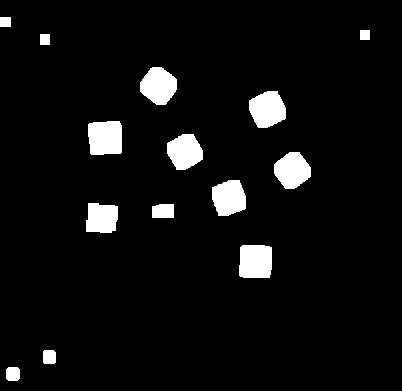
\includegraphics[width=.25\textwidth]{final_mask2.png}            
	}                                                                             
\end{figure}

The code for getting the mask and processing it can be seen below.
%
\begin{lstlisting}[ language = Matlab,
caption  = {MATLAB code to get the mask that contains the blocks.},
label    = list:mask ]
% Find the blocks in the image
saturation=imgaussfilt(saturation,'FilterSize',9);  % First, find coloured blocks using the saturation channel
colour_mask=saturation>MyParameters.COLOR_THRESHOLD*ones(y,x);
black_mask=value<MyParameters.BLACK_THRESHOLD*ones(y,x); % Then, the black blocks using the value channel
final_mask=black_mask | colour_mask; % Join masks for coloured blocks and black blocks
se = strel('square',5); % Procesing of the mask to fill holes and eliminate noise
final_mask=imopen(final_mask,se);
se = strel('square',5);
final_mask=imclose(final_mask,se);
\end{lstlisting}

Once the mask is enhanced, each of the objects can be labeled to be analyzed one by one. It is worth mentioning that only the objects that have an area larger than a threshold of 250 pixels are considered for future processing. This helps removing the effect of any persistent noise blob that survived the morphology operations.

The position of each brick in the picture is then found using the centroid of the pixels corresponding to each object, as seen in \autoref{fig:centroids}.
%
\begin{figure}[H]
	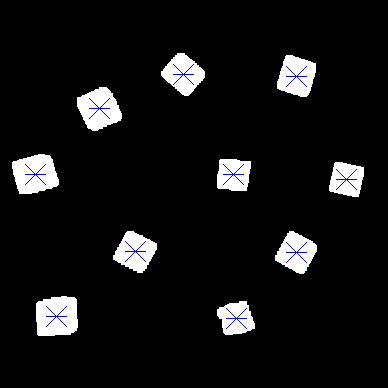
\includegraphics[width=0.3\textwidth]{figures/centroids.png}
	\caption{Centroids of the different objects in the mask (blue marks).}
	\label{fig:centroids}
\end{figure}

The object and it properties are identified using the following commands in MATLAB:
%
\begin{lstlisting}[ language = Matlab,
caption  = {MATLAB code to get the objects and their properties.},
label    = list:centroid ]
% Identifying objects and their properties
objects = bwconncomp(final_mask);           % Label the objects
area = regionprops(objects,'Area');         % Calculate the areas of the objects
centroid = regionprops(objects,'Centroid'); % Find centroid of the objects
pixelList=regionprops(objects,'PixelList'); % Fins the pixels of each block
nobjects=length(centroid);                  % Number of objects found
\end{lstlisting}

Once the position of the brick in the image is known, it is necessary to identify its color. This is done by looking at a small region around the center of each brick in the hue channel. The mean hue of the pixels in the region is compared to hue reference values corresponding to yellow, green, blue and orange. The region used in the algorithm is a square centered in the centroid and with 5 pixels on each side. The hue values used were obtained by examining images of the bricks taken in similar conditions leading to 0.12 for yellow, 0.05 for orange, 0.61 for blue, and 0.44 for green. All of them are represented in a [0,1] range. The color of the object is then selected as the one closer to the mean of the region. 

The color identification code can be seen below:
%
\begin{lstlisting}[ language = Matlab,
caption  = {MATLAB code find the color of the brick.},
label    = list:color ]
% Get a mask of the object in the hue channel and on the black mask
cent_y=round(centroid(i).Centroid(2));
cent_x=round(centroid(i).Centroid(1));
region_hue=hue(cent_y-MyParameters.MASK_SIDE:cent_y+MyParameters.MASK_SIDE,cent_x-MyParameters.MASK_SIDE:cent_x+MyParameters.MASK_SIDE);

% Sort by colour and store centroid position and orientation
if (mean(mean(region_blackmask,1)) >= 0.8)
     blocks.black = [blocks.black; [cent_real angle]];
else
    meanhue=mean(mean(region_hue));
    [~,color_index]=min(abs(meanhue*ones(1,length(colorlist))-colorlist));
    switch color_index
        case 1
            blocks.yellow = [blocks.yellow; [cent_real angle]];
        case 2
            blocks.green = [blocks.green; [cent_real angle]];
        case 3
            blocks.blue = [blocks.blue; [cent_real angle]];
        case 4
            blocks.orange = [blocks.orange; [cent_real angle]];
    end
end
\end{lstlisting}

The last information that should be extracted by the algorithm is the orientation of the object. It is based on and edge detection followed by a Hough transform for lines. Since the image is already binary, \autoref{fig:object_mask}, the edges can be detected by calculating the difference between the image and a dilation of it. The result can be seen in \autoref{fig:edges}.
%
\begin{figure}[H]
	\captionbox  %<--use captionbox instead if no global caption is needed
	{
		Mask for one of the objects.              
		\label{fig:object_mask}                                  
	}                                                                 
	{                                                                  
		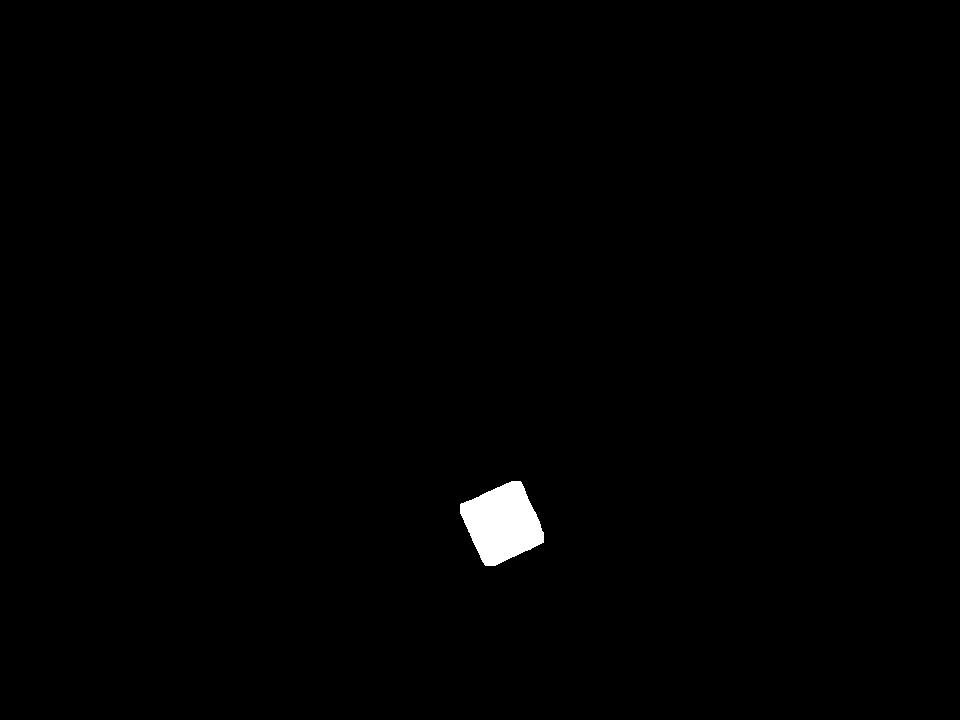
\includegraphics[width=.25\textwidth]{figures/object_mask.png}         
	}                                                                    
	\hspace{5pt}                                                          
	\captionbox
	{       
		Edges found in the object by the difference of the original mask and a dilated one.
		\label{fig:edges}                                     
	}
	{
		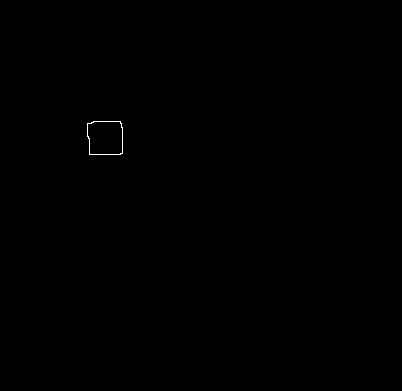
\includegraphics[width=.25\textwidth]{edges.png}            
	}                                                                              
\end{figure}

Once the edges are found, the Hough transform is used to find the lines with a minimum length of 20 pixels. The orientation of each brick then is defined as the angle of the longest line found with respect to the horizontal axis, see \autoref{fig:object}. 
%
\begin{figure}[H]
	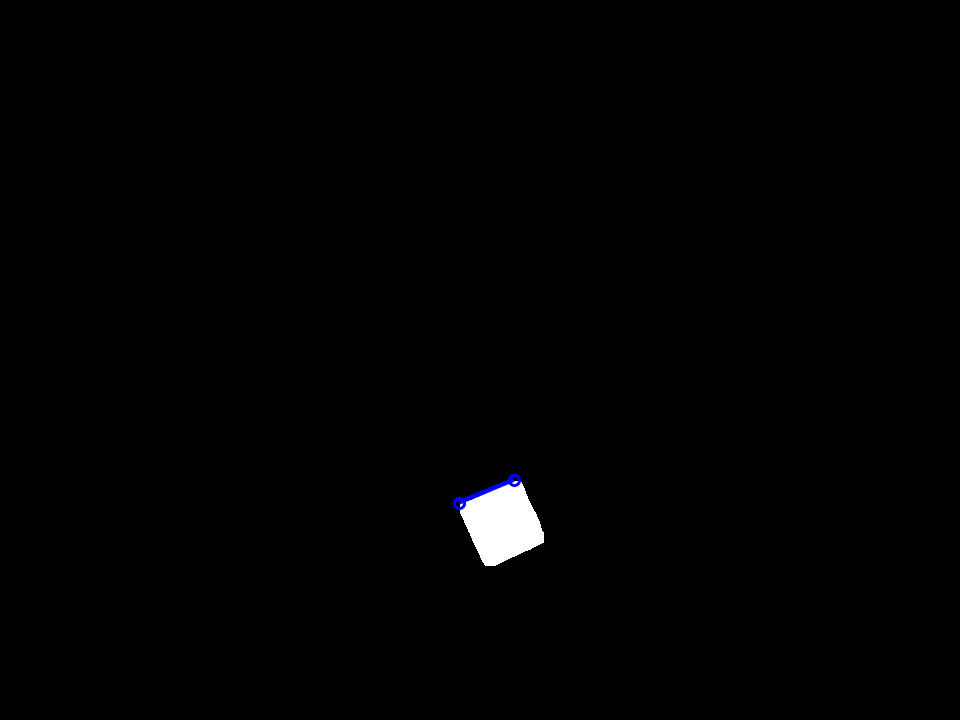
\includegraphics[width=0.25\textwidth]{figures/object.png}
	\caption{Largest line in the object marked in blue.}
	\label{fig:object}
\end{figure}

Since the orientation needs to be expressed in workspace coordinates, the two points that defines that line are transformed to scene coordinates using the transformation matrix defined in \autoref{sec:camera}. This is straightforward for the position as
%
\begin{flalign}
	\begin{bmatrix}
		U \\
		V \\
		W
	\end{bmatrix}
	=H
	\begin{bmatrix}
		x \\
		y \\
		1
	\end{bmatrix}
    ; \ \ \ \
    X_\mathrm{s}=\frac{U}{W}; \ \ \ \
    Y_\mathrm{s}=\frac{V}{W}
\end{flalign}

The algorithm for getting the position and orientation can be seen in \autoref{list:pos}.
%
\begin{lstlisting}[ language = Matlab,
caption  = {MATLAB code to get the position and orientation.},
label    = list:pos ]
cent_real=MyParameters.H*[cent_x,cent_y,1]'; % Transform the position to real coordinates
cent_real=cent_real(1:2)'/cent_real(3);
edges=imdilate(object_mask,se)-object_mask; % Find the edges of the object mask by substacting the image and its dilation
[H,theta,rho]=hough(edges,'RhoResolution',1,'ThetaResolution',5); % Find lines in the resulting image using the Hough transform
P = houghpeaks(H,16,'threshold',ceil(0.1*max(H(:))));
lines = houghlines(edges,theta,rho,P,'FillGap',10,'MinLength',20);
nlines=length(lines);
dist=zeros(1,nlines);
for k = 1:1:nlines % The longest line is stored and used to define the orientation
    dist(k) = norm(lines(k).point1 - lines(k).point2);
end
[~,max_dist]=max(dist);

xy1_real=MyParameters.H*[lines(max_dist).point1 1]'; % The position of the points that define the line are transformed
xy1_real=xy1_real(1:2)'/xy1_real(3);                 % to real positions using the projection matrix
xy2_real=MyParameters.H*[lines(max_dist).point2 1]';
xy2_real=xy2_real(1:2)'/xy2_real(3);

xy_real = [xy1_real; xy2_real];
angle = atand((xy_real(2,2)-xy_real(1,2))/(xy_real(2,1)-xy_real(1,1))); % The angle with respect to the base x axis is found using this two points
\end{lstlisting}

At this point, each brick is identified by its position in the image, its color and its orientation in workspace coordinates.

\section{Pick and Place Movement}
The strategy for picking a piece and placing it in its final destination is composed by several movements. This operation is programed in the MATLAB function located in \lstinline[style=matlabinline]{PickPlace.m}

Initially, the robot is placed on top of the brick that is to be picked. This also includes rotating the gripper to the appropiate orientation. Then, the gripper is moved down vertically until the height is correct and the brick can be grabbed. Finally, the tool with the brick move up vertically finishing the pick operation. \autoref{list:pick} shows how this sequence looks like when programed in MATLAB.
%
\begin{lstlisting}[ language = Matlab,
caption  = {MATLAB code to perform the pick instruction.},
label    = list:pick ]
% Move to the initial pose with some heigth, go down, grab the brick and go up
% again
moveLinear(kuka,x,y,z+MyParameters.HEIGHT,a,b,c,vel)
moveLinear(kuka,x,y,z,a,b,c,vel)
closeGrapper(kuka)
moveLinear(kuka,x,y,z+MyParameters.HEIGHT,a,b,c,vel)
\end{lstlisting}

After the brick is picked, it is placed in its final destination following similar movements. The tool moves to the final location with the right orientation, then moves down, releases the brick and moves up vertically, ready to start a new pick operation with another block. In MATLAB, these movements are programed as in \autoref{list:place}.
%
\begin{lstlisting}[ language = Matlab,
caption  = {MATLAB code to perform the place instruction.},
label    = list:place ]
% Move to the pose with some heigth, go down, release the brick and go up
% again
moveLinear(kuka,x,y,z+MyParameters.HEIGHT,a,b,c,vel)
moveLinear(kuka,x,y,z,a,b,c,vel)
openGrapper(kuka)
moveLinear(kuka,x,y,z+MyParameters.HEIGHT,a,b,c,vel)
\end{lstlisting}